\section{LHCb Experiment}

The LHCb experiment is one of the 7 experiments located on the Large Hadron Collider. It was built in order to search for indirect evidence of new physics phenomona through the study of CP violation and rare decays for hadrons that contain b and c quarks.

In proton collisions provided by the LHC heavy quark pairs are predominantly produced at small angles to the beam pipe. The dominant production mechanisms that produced bbbar pairs are quark anti-quark annihilation, gluon-gluon fusions and  gluon splitting as shown in the Feynman diagrams in Figure X. There must be some other reason why these processes lead to the quarks being boosted along the beam pipe and I shall explain that here. Once the bbbar pairs are produced the quarks hadronise(?), in to Bs, Bd, B+ and many others and the decays of these hadrons have some specific characteristics. B-mesons have long lifetime around 1 ps therefore travel ~1cm from the interaction vertex where they were produced before decaying at a secondary vertex. Good identification of the secondary vertices is necessary to determine that the B hadrons decay into. Since b quarks are heavy quarks, the hadrons they for can decay into a large range of differnt particles from light particle such as electrons and photons to heavier particles like kaons, muons and D meson. Therefore a good detector for b physics needs to be able to identity a range of decay produced to accurately reconstruct what actually decayed. The experiment was designed around the production characteristics of bbbar pairs and to enable precise measurements of b hadron decays. 

The LHCb experiment was built as a single arm forward spectrometer, with an angular coverage of 10 to 300 mrad in the vertical direction and 10 to 250 mrad in the horizontal direction relative the the beam pipe. This angular coverage what chosen to exploit the small angles relative the the beam pipe that bbbar pairs are produced at. A cross-section of the detector is shown in Figure X, where a right handed coordinate system is used. Protons collide at the interaction point on the left hand side of the diagram, the products of the collisions then travel through the detector leaving information in the different sub detectors along the length of the detector. The information deposited in the sub detectors are reconstructed to determine what happened in the proton collisions. The sub detectors can be classified in to two main categories; tracking system and particles identification system .

The tracking system is make up to the vertex locator (VELO), the magnet, the TT and the tracking stations T1-3. The VELO is designed to provide precise tracking measurements to identity the primary and secondary vertices characteristic of b-hadron decays in order to determine accurate lifetimes of b-hadrons. The magnet and tracking stations are combined to give high momentum resolution which is necessary to achieve good mass resolution which is used to distinguish between different b hadrons and separate signal and background decays.
%Need good decay time resolution if we are to measure the rapidly oscillatin Bs system.
The particle identification detectors provide complementary information about the identity of particles passing through them which enables the many different decay products of b-hadrons to be identified and the hadron to be accurately reconstructed. The RICH detectors provide information about these types of particles, the two calorimeters give informations that separates electrons, positrons and photons and from hadrons. Finally the muons stations at the furthest point from the integration point identify muons as the name suggests. 

The measurement of of decays of heavy hadrons requires accurate reconstruction of secondary vertices, this is achieved in part by the tracking systems however another aspect of the LHCb experiment deigns that enables this is the luminosity the experiment operates at. The LHC was designed to deliver a luminosity of X, proton collisions at this luminosity leads to a large amount of pile up. Pile up is stuff from the decay that is not interesting and is close to the beam pipe, therefore in the LHCb acceptance and makes it hard to accurately reconstruct secondary verticies. Therefore LHCb operates at a lower luminosity of ~ X in order to reduce the amount of pile up and enable accurate reconstruction of b hadron decays. 

The tracking and PID systems are described in the following sections as well as the way events are selected at LHCb and processed and analyses. 



\begin{figure}[tb] 
  \centering    
  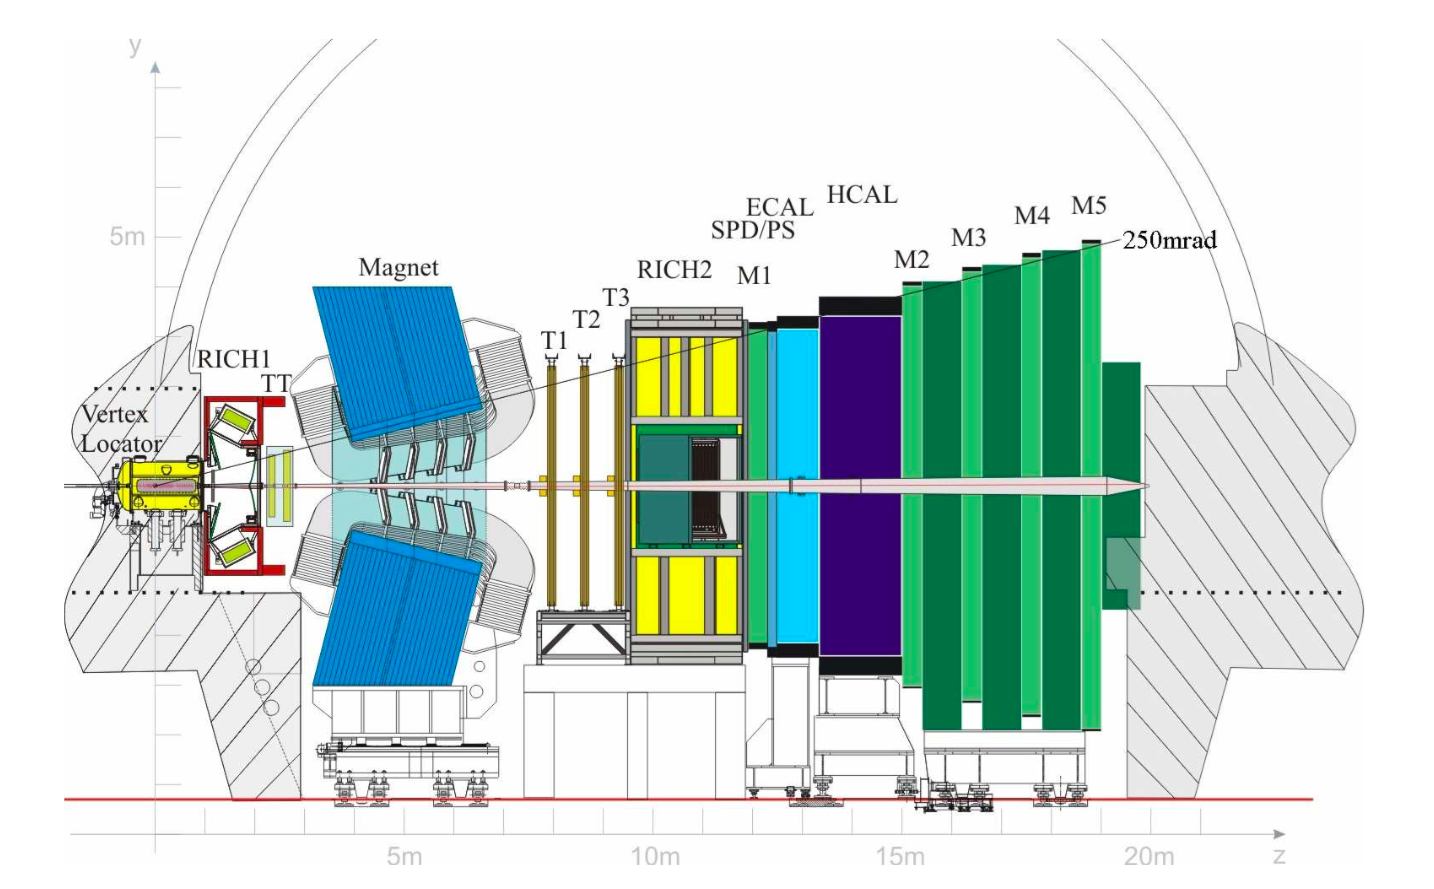
\includegraphics[ width=1.0\textwidth]{./Figs/LHC_LHCb/lhcb.png}
  \caption{Cross section of the LHCb detector \cite{Alves:2008zz}.}
  \label{fig:LHCb_detector}
\end{figure}



\begin{figure}[tb] 
  \centering    
  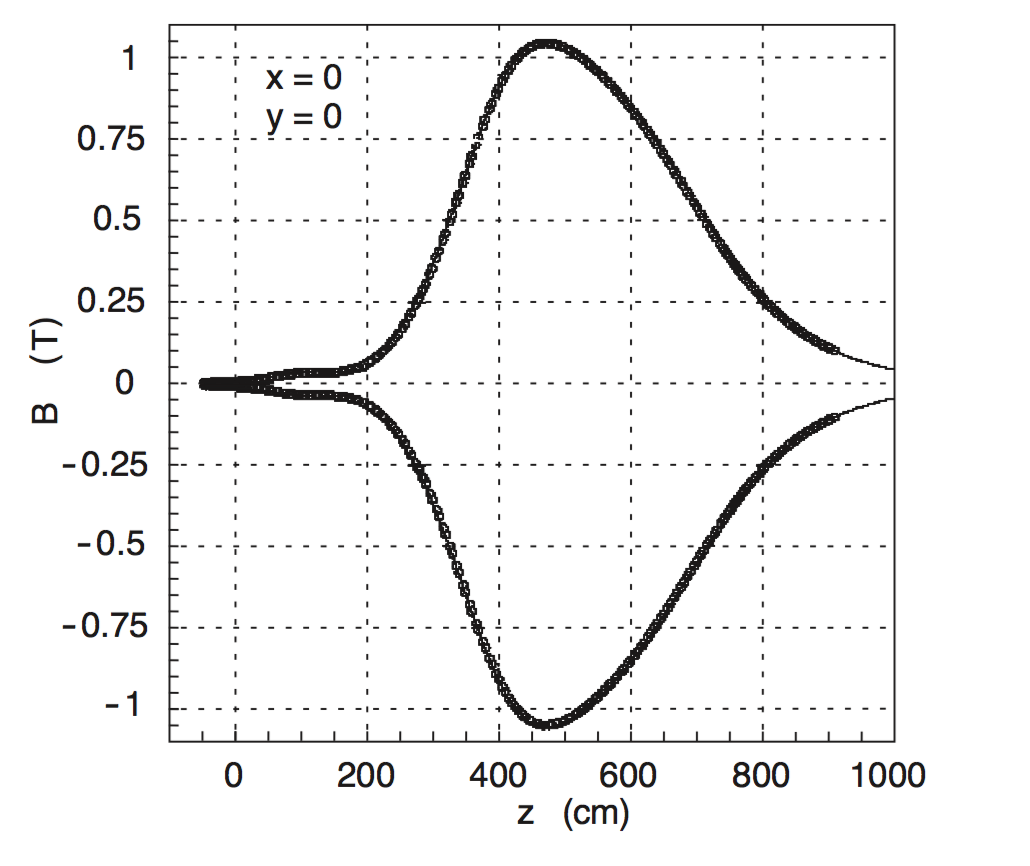
\includegraphics[ width=1.0\textwidth]{./Figs/LHC_LHCb/Magnet_field.png}
  \caption{Magnet field \cite{Alves:2008zz}.}
  \label{fig:LHCb_detector}
\end{figure}




\begin{figure}[tb] 
  \centering    
  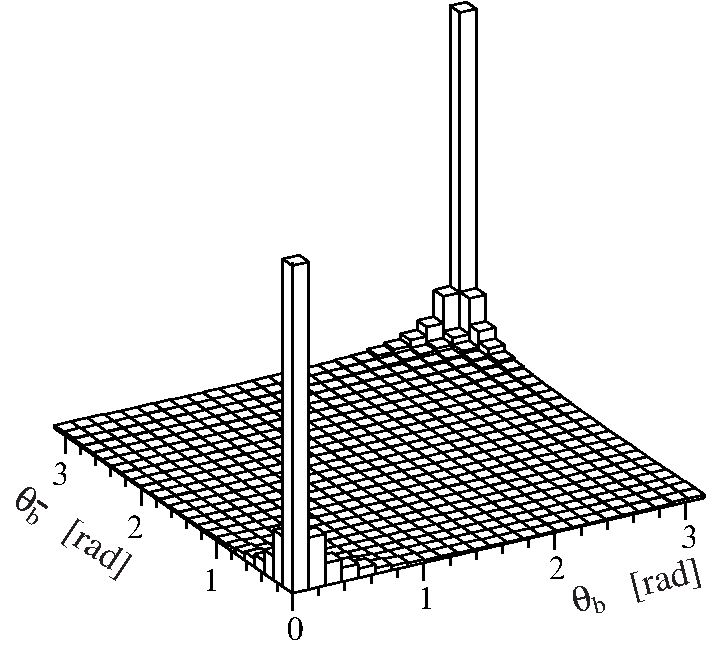
\includegraphics[ width=1.0\textwidth]{./Figs/LHC_LHCb/b_distrib_lhcb.pdf}
  \caption{Simulated angular distribution for b-quark production at the LHC, angles are relative the the beam pipe with $\theta =0$ in the forward direction and$\theta = \pi$  in the backward direction \cite{Amato:1998xt}.}
  \label{fig:LHCb_detector}
\end{figure}


\subsection{Tracking}


The tracking system within the LHCb experiment consists of the VELO, the magnet and the tracking stations which are the Tracker Turicensis (TT) and three tracking stations (T1-3). The VELO surrounds the interaction point and the magnet is between the TT and the tracking stations (T1-3). Together they work to provide precise information of the passage of charged particles though the detector which is needed for accurate analysis for b-hadron decays. The VELO gives precise information about the primary and secondary vertices where as the tracking stations give full track reconstruction. 

\subsubsection{VELO}
The VELO is a silicon detector that surrounds the interaction point. It’s main goal is to provide precise information about the interaction vertices and secondary decay vertices of particles produced in proton collisions. Important to give us lifetimes and impact parameters. The VELO covers the full LHCb angular acceptance.

The VELO is made up of 2 identical halves, each half consists of 21 stations each containing 2 silicon sensors arranged along the beam pipe. The arrangement is shown in figure X. The z distribution is such that the flow covers the full LHCb acceptance and a charged track within the acceptance will pass through at least 3 stations. In each station the 2 sensor measure different coordinates, one measures the r coordinates of charged particles and the other measures the phi coordinates they are distributed along the length of the VELO. The r, phi and z cordidiates are used to reconstruct charged particle trajectories. Cylindrical coordinates were chosen to allow for fast reconstruction for particle trajectories in the VELO so that the can be used in the trigger. Figure X shows examples of the two types of sensor in the VELO. There is a small hole in the centre of the sensors to let the beam through.

The momentum resolution of charged tracks depends on multiple scattering, therefore to allow for good momentum resolution to be determine in the other tracking stations, the VELO is kept in a vacuum so reduce it’s material budget. Each half of the VELO is enclosed inside an aluminium box, this keeps the VELO in a  vacuum the VELO but it also shields the electronic readouts of the VELO from radio frequencies which are generated by the beam. The VELO material budget comes to 17.5 $\%$ of a radiation length.

Excellent vertex resolution is required in the VELO, to achieve this the sensors in the VELO need to be as close as possible to the interaction point. This is achieve by having 2 separate halves to the VELO. During data taking when the VELO is record the location of primary and secondary vertices the veto sensor at only 8mm from the beam axis. However during the injection phase of the beam the width of the beam is much greater, therefore the 2 halves of the VELO can retract so that they are 3cm from the nominal beam axis which keeps them safe from radiation damage. This is all shown in Figure X. The two half of the veto aren’t aligned, they are displaced by 150 mm in the z direction so that when the VELO is closed, the sensors in each half overlap, this helps with detector alignment and reduced edge effects.


Furthermore the interaction point is within the velo, there are sensors up stream of the interaction point which allows for accurate reconstruction of PVs.


Another feature if the VELO is that is can act a veto for high pile up events. There are 2 VELO sensor upstream of the interaction point that act a pile up vetoes, they given information to the trigger about how many pp interactions there were with each bunch crossing and help to select only what we’d be good a reconstructing. ( it rejects events with a large number of pp interactions)

Overall the VELO gives such and such precision.  vertex resolution in the transverse plane 10-20 mircons, in the z directions 50-100 microns depending on the number of tracks in the vertex. %The VELO is also important the impact parameter resolution and decay time resolutions.  (This may go at the end so that everything for tracking is together?) best resolution is 4 micrometers which allows a lifetime measurement of 50 fs. (Performance paper)


\begin{figure}[tb] 
  \centering    
  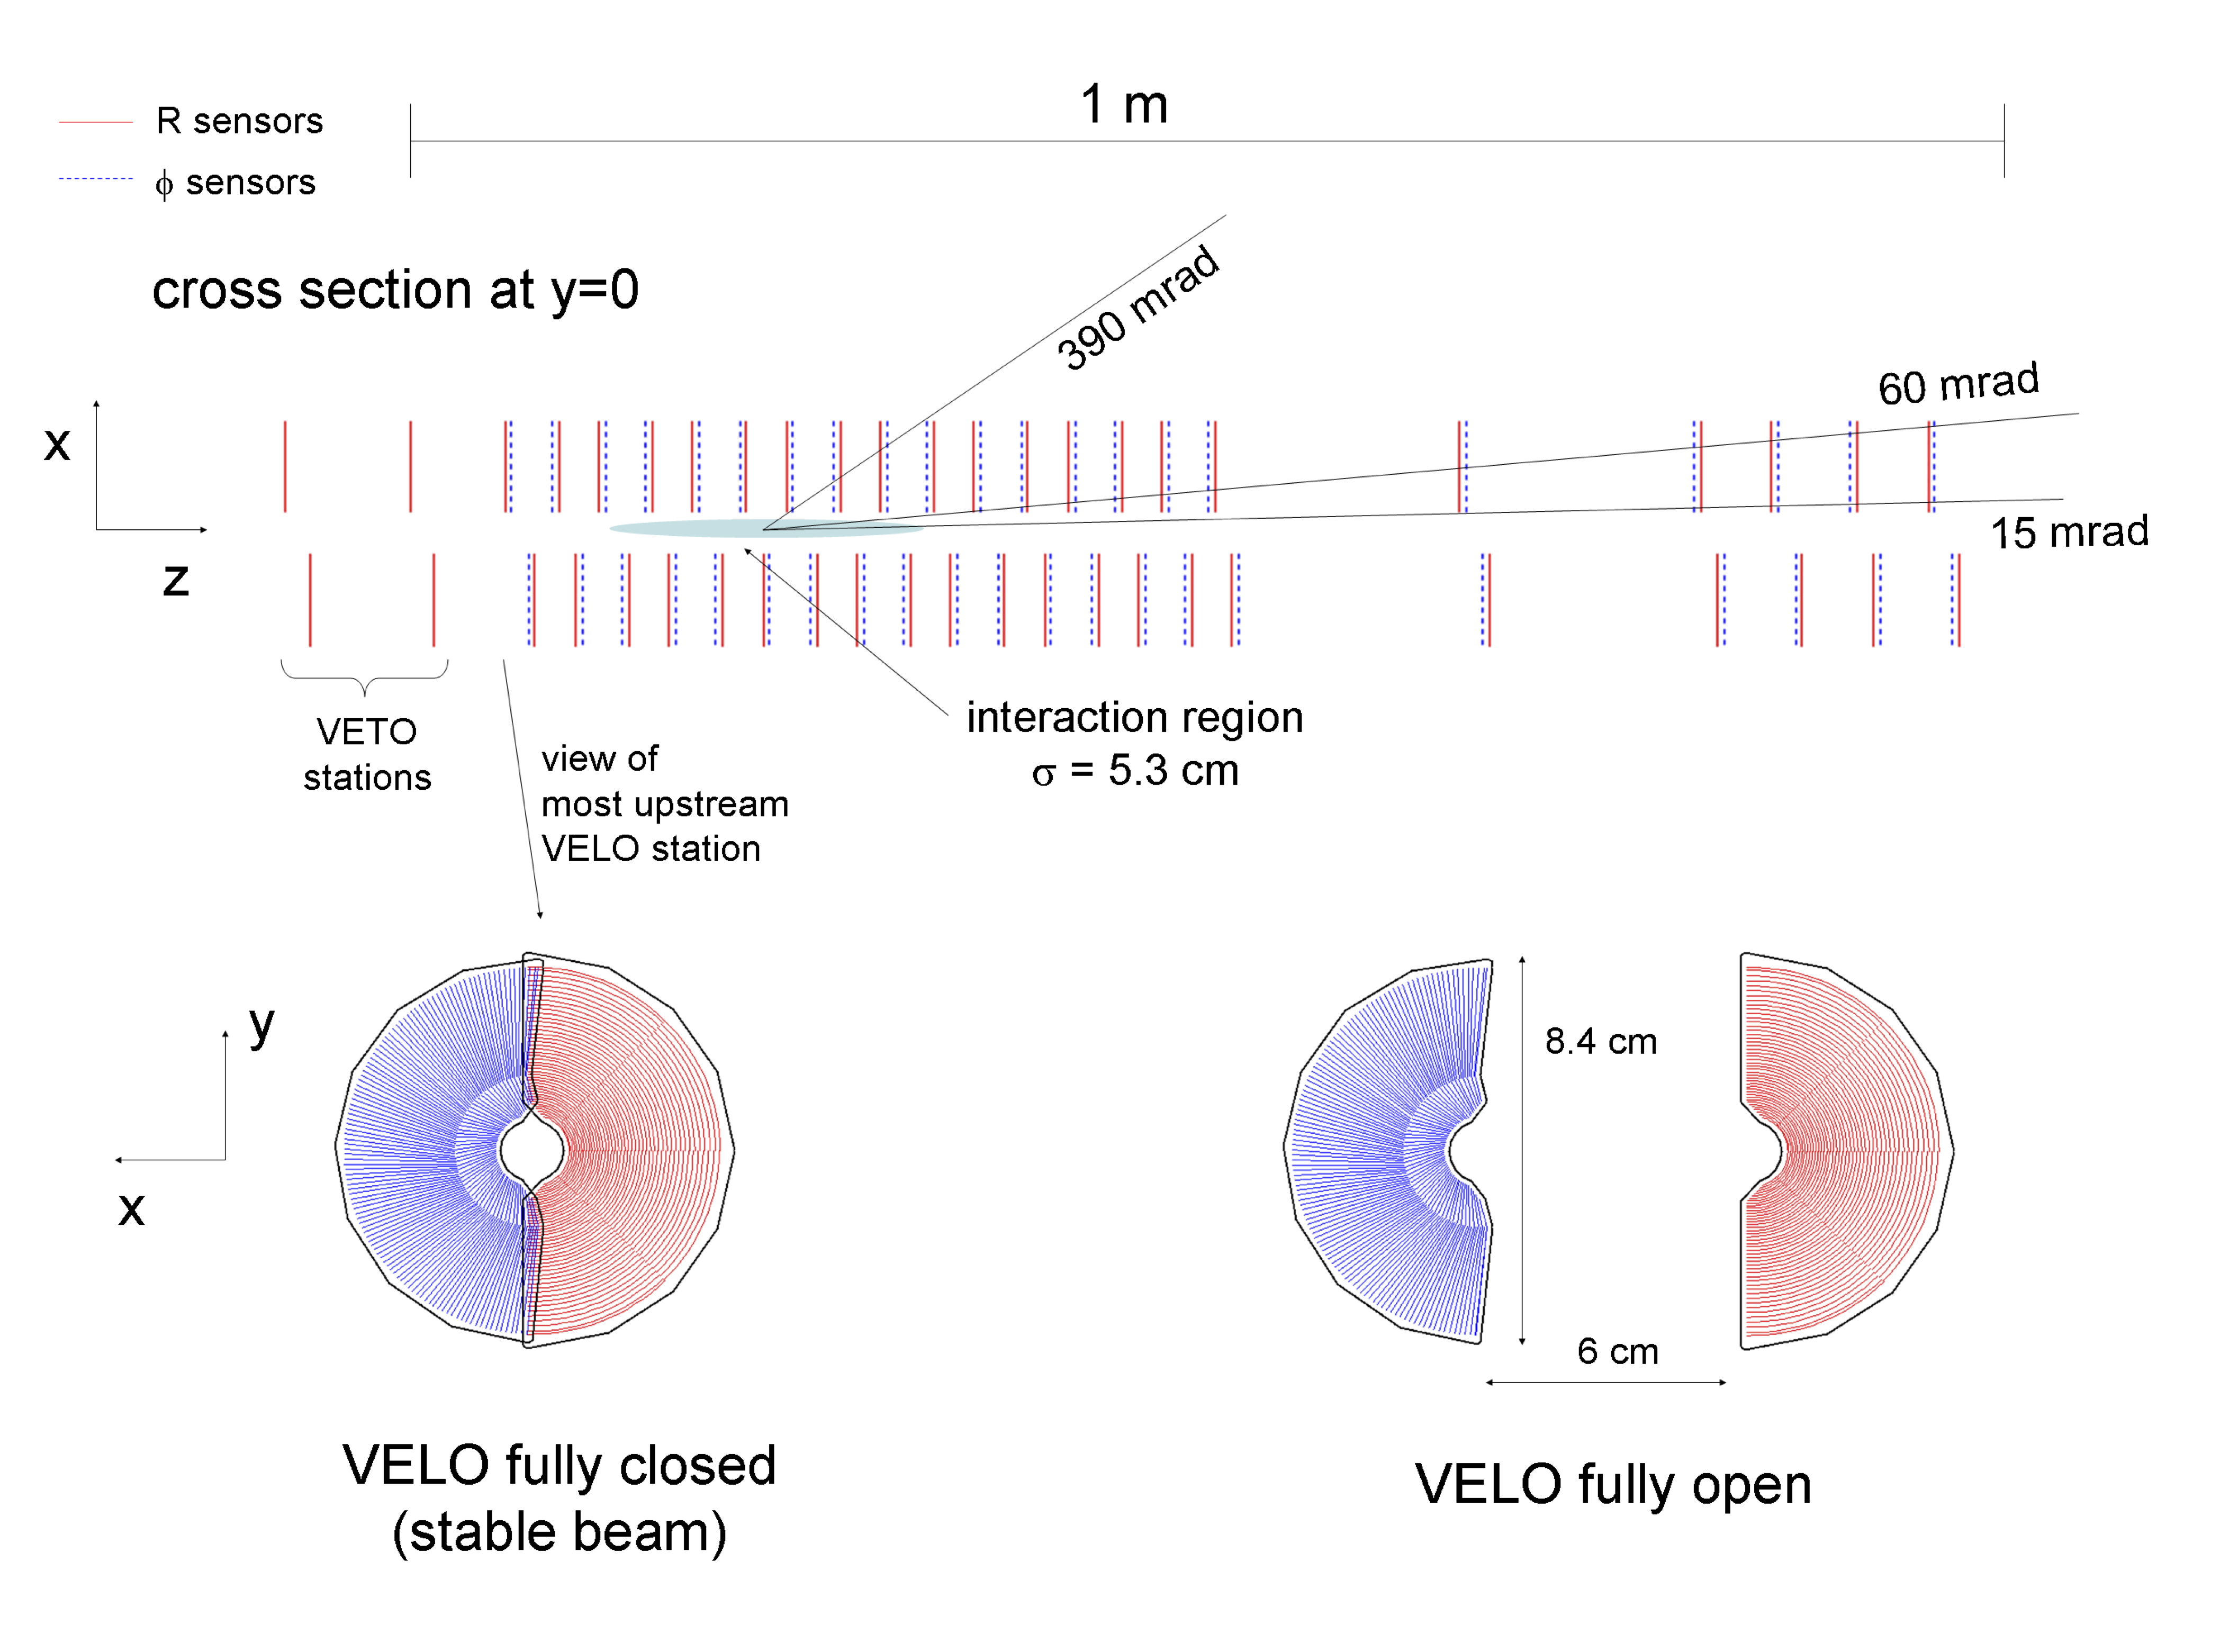
\includegraphics[ width=1.0\textwidth]{./Figs/LHC_LHCb/velo.png}
  \caption{The velo \cite{Alves:2008zz}.}
  \label{fig:velo}
\end{figure}

\begin{figure}[tb] 
  \centering    
  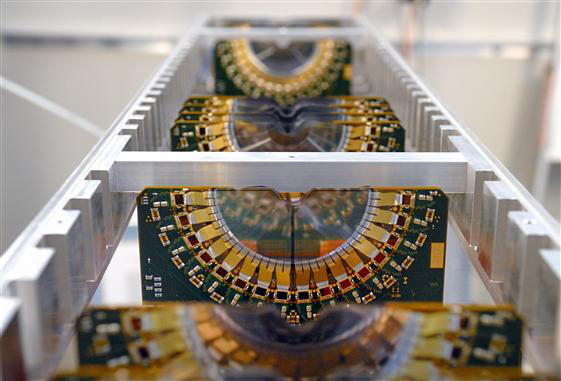
\includegraphics[ width=1.0\textwidth]{./Figs/LHC_LHCb/Velo_photo.jpg}% ./Figs/Detector/Velo_photo.jpg}
  \caption{The velo Soure: LHCb.}
  \label{fig:velo_photo}
\end{figure}

\begin{figure}[tb] 
  \centering    
  
\includegraphics[ width=1.0\textwidth]{./Figs/LHC_LHCb/placeholder.jpeg}
  \caption{The velo sensor \cite{Alves:2008zz}.}
  \label{fig:velo_sensor}
\end{figure}

\subsubsection{Tracking Stations} 
The LHCb experiment has 4 tracking stations in addition to the VELO, the Tracker Turicensis (TT) which is located upstream of the magnet and the tracking stations T1 to T3 located down stream of the magnet. These tracking stations provide complementary tracking information to that of the VELO and the presence of the magnetic field within the tracking stations allows the momentum of charged particles to be determined. 



The TT is made up of 4 layers of silicon trackers spaced 27 cm apart that covers the full LHCb angular acceptance. The TT is located just within the influence of the magnetic field of the dipole magnet, which provides the detector with 2 main purposes. Firstly, the TT tracks the passage of charged particles with high momentum to enable high momentum resolution for tracks when combined with the other tracking stations. In order to achieve this the TT has a resolution of 50 $\mu$m for a single hit which means that multiple scattering rather than detector resolution is the limiting factor for the momentum resolution. The second purpose of the TT is to record tracks of low momentum particles that are then swept out of the detector acceptance as they continue through the magnetic field. 
%Information from just the TT and the VELO can provide an momentum accuracy of ~ 20 $\%$. 
%active area of 8.4m^2


The 3 tracking stations T1-3 are split into two sections, they are each composed of an Inner Tracker (IT) made of silicon and an Outer Tracker (OT) composed of straw tubes. 
The increase in size of the tracking stations between the TT and the T3 in order that the detectors cover the required angular acceptance is very large.  The TT is 150 cm by 130 cm where as the T3 station is 600cm by 490 cm, this is illustrated in Figure X. Therefore due to cost reasons the tracking stations cannot be whole made of silicon. 

The IT is very similar in design to the TT, it is make of 4 layers of silicon trackers in each station with a track resolution of 50 $\mu$m.
%and has an active area of 4.0m2. 
The silicon trackers are arranged in a cross shape around the beam pipe, as shown in Figure X, although the cover less than 2$\%$ of the tracking stations 20$\%$ of tracks pass through them. This allows the occupancy of the OT to be less than 10$\%$ so that it can be made of something other than silicon and still give good overall momentum resolution. The OT of each tracking station is made of 2 staggered layers of straw tubes, they cover the remaining area required for cover the LHCb full angular acceptance which includes tracks bend by the magnetic field of the magnet. The tubes have a fast drift time of 50 ns which enables a better than 200 $\mu$m track resolution. 


\subsubsection{The Dipole Magnet}
A warm dipole magnet is used to measurement the momentum of charged particles travelling through the LHCb detector. In a magnetic field the trajectories of charged particles are bent and from the radius of curvature of the particle track the momentum of said particle can be determined.

The magnet is located between the TT and the tracking stations T1-3 and it’s field covers the full LHCb acceptance. The field is in the vertical direction therefore bending tracks in the horizontal direction. The magnet was designed so that it’s strength in the RICH detectors is negligible (less than 2 mT) and to have the largest strength possible between the TT and T1-3. Figure X shows a plot of the magnet strength overlaid on the detector. A small magnetic field is achieved in the RICH detectors by shielding. The magnet was therefore designed to have an integrated field strength is 4Tm for track that travel 10m and the peak strength is 1.1T. % I should maybe mention the measurement of the field and how it had to be accurate (with Hall probes) in order to get good momentum resolution but I don’t want to.

The polarity of the magnetic field is periodically switched therefore bending charged tracks in opposite directions. This is done so that left-right detection asymmetries can be measured and it helps with the systematic uncertainties of CP violation measurements. % These are not relevant for B2mm.

\subsubsection{Track resconstruction and Preformance of the tracking}


The information left by the passage of charged particles in each of the VELO, TT and T stations are combined using track reconstruction algorithms for determine the passage of charged particles through the detector. The algorithms start with either segments of tracks in the VELO or the T stations as seeds and then extrapolate using these segments into the other tracking detectors joining tracking in specific search windows in each detector. The rescontructed tracks are classified into five different types depending on what signature they left in each detector. The different types of tracks are illustrated in Figure X. 

VELO tracks come from particles that only leave information in the VELO, these tracks usually are at a large angle or are travelling backwards and are useful in reconstructing primary vertices.

Upstream tracks are formed by low momentum particles that are only observed in the VELO and the TT because they are them swept out of the detector acceptance by the magnetic field. These tracks have a poor momentum resolution but are useful for understanding backgrounds and pattern recognition in the RICH 1 which is located between the VELO and the TT provided the particles have sufficient momentum to be seen in the RICH.

Downstream tracks come from decay of the long lived particles, these particles do no leave information in the VELO only the TT and T stations. 

T tracks are tracks that only cross the T1-3 station and are formed from particles created from interactions with the material in the detector. Similarly to upstream tracks, T tracks can help to understand backgrounds and pattern recognition in the RICH2 which is located just before the T stations.

Long tracks are the most useful for physics analyses because they are formed from information left in the VELO, TT and T1-3 stations and consequently these tracks have the best momentum resolution.

The efficiency to correctly reconstruct tracks depends of different parameters of the events, such as the momentum to the particle producing the track, for long tracks they are correctly reconstructed on average of 96$\%$ of the time as shown in Figure XX for Run 1 data. 

Tracking efficiencies were measured using tag and probe method with Jpsi2MuMu, the average effieicny is better than 95 $\%$ for the mometum range 5 - 200 GeV and pseuoradify range 2-5 for Run 1. % (this is pretty much a quote from the paper. There are lots of plots in the paper so I think I should leabe them out!
Once the segments of the track have been found the trajectory is fitted with a Kalam fitter with takes into account multiple scattering and energy loss within the detector. For each track the fitter returns the chi2/ndof for each track which is a measure of quality for the track. In LHCb this parameter is used to ensure that only ‘good’ tracks are used in analyses. 

Inevitably every track that is reconstructed is not correct, there are two main types of incorrectly reconstructed tracks. The first is clone tracks that occur when the two tracks share many hits in common, when this happens the track with the highest number of total hits it used and the other is discarded. The second type of incorrect track are ghost tracks when segments in different detectors are incorrectly joined together, this can happen with tracks in the VELO and T1-3 stations, the number of times that this happened depends on the multiplicity of an event. These tracks are remove by cutting on the output of a neural network that returns a probability of how likely a track is to be fake.



Once the tracks have been reconstructed this allows the computation of different parameters that are necessary for the identifying different b hadron decays. The performance of the tracking system has been studied of Run 1 data \ref{ performance paperS}. The tracking system provide measurement of the momentum of the charged particles that it tracks, good momentum resolution is required in order to obtain good mass resolution which is necessary to identify different  b hadrons and to distinguish between signal and background events. The momentum resolution of long tracks is shown in figure X OR the momentum resolution is $\delta$p/p = X - Y $\%$ which depends on the momentum of the reconstructed track. 


The tracking system allows accurate reconstruction of primary verticies, this is necessary to measure time dependant processes, lifetimes and identify decaying particles. It was particular important for LHCb so that is could measure the rapidly oscillation Bs system. The PV resolution has been measured on 2012 data and varies with the number of tracks used to reconstruct the vertex, on average the vertex resolution transverse to the beam is between 10 and 25 mum and parallel to the beam is  between 50 and 150 mum for the z direction as shown in figure X for 2011 data. %Ref veto paper.



The impact parameter is another important variable, it measure the distance of closest approach of a track to the PV, long lived particles tend to have a large IP wrt to PV because they travel before they decay. Good measurements of the IP help to remove prompt backgrounds. The IP resolution depends on the momentum of the particles and figure X shows the IP resolution for 2012 data, for a track with transverse momentum of 1 GeV/c is has an IP resolution of 35 mum.


Finally, the measurement of lifetime of b hadrons at LHCb needs accurate decay time measurements but more importantly to understand the rapidly oscillating Bs system good decay time resolution is needed. To reconstruct the decay time information about particle momentum and decay length, how far the particle travelled before it decays are needed. Therefore good PV resolution and moment resolution are needed. The LHCb detector achieved typically 50 ns resolution on the decay time. 


VELO performance paper \cite{LHCbVELOGroup:2014uea}.
LHCb preformance paper \cite{Aaij:2014jba}.
Tracking effieicny paper \cite{Aaij:2014pwa}.

\begin{figure}[tb] 
  \centering    
  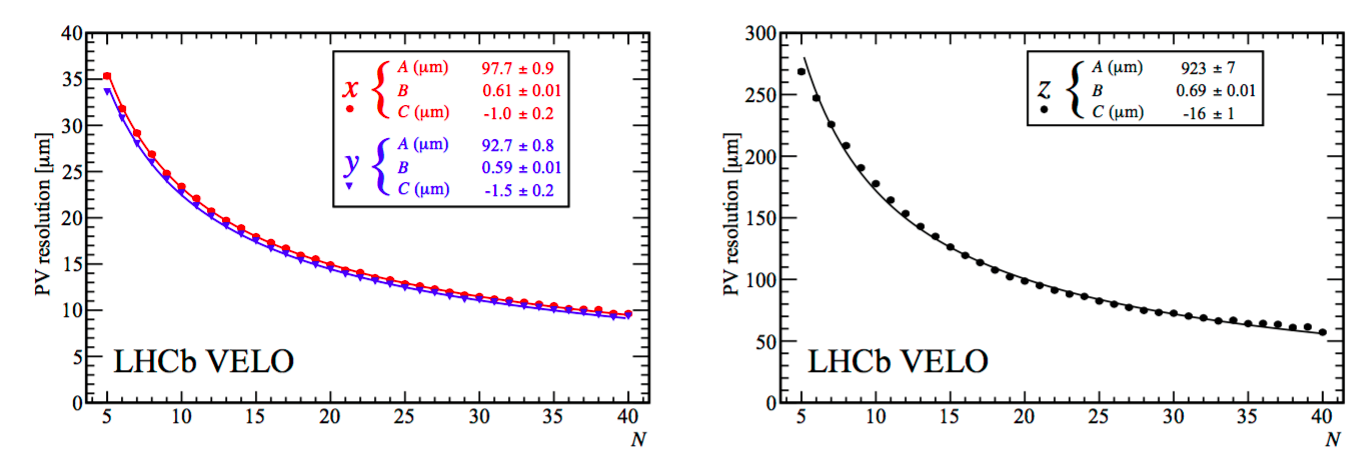
\includegraphics[ width=1.0\textwidth]{./Figs/LHC_LHCb/Velo_vertex_resolution.png}
  \caption{Velo prefomance. Source: \cite{LHCbVELOGroup:2014uea}.}
  \label{fig:types_of_tracks}
\end{figure}



\begin{figure}[tb] 
  \centering    
  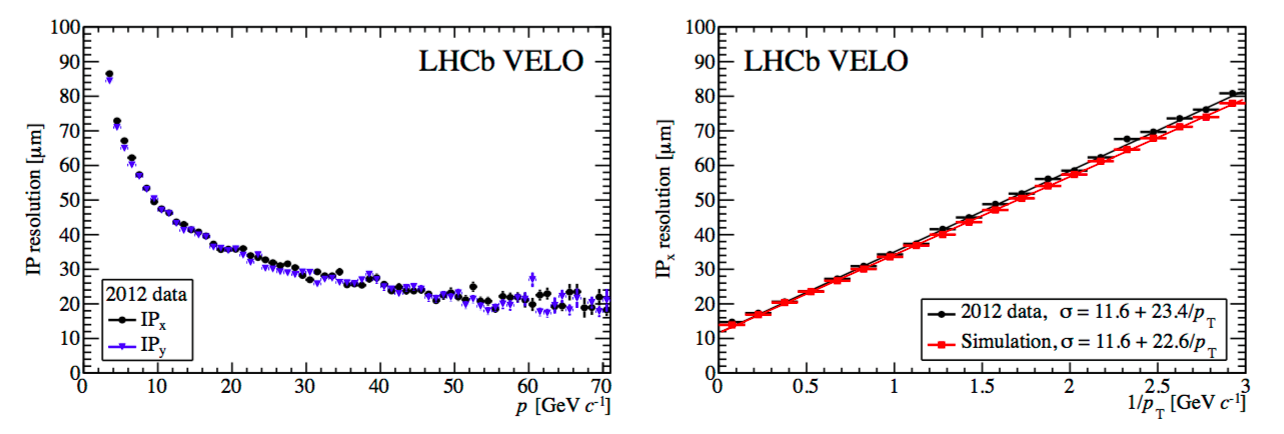
\includegraphics[ width=1.0\textwidth]{./Figs/LHC_LHCb/Velo_IP_resolution.png}
  \caption{Velo prefomance. Source: \cite{LHCbVELOGroup:2014uea}.}
  \label{fig:types_of_tracks}
\end{figure}


\begin{figure}[tb] 
  \centering    
  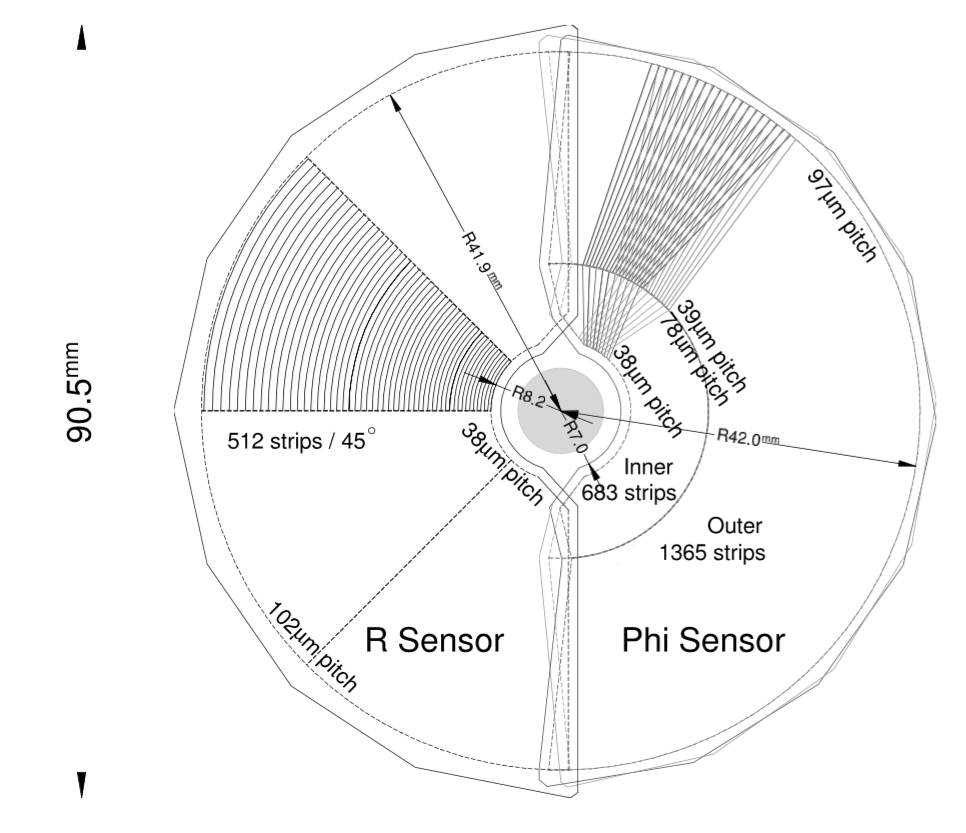
\includegraphics[ width=1.0\textwidth]{./Figs/LHC_LHCb/Velo_sensor_diagram.png}
  \caption{Velo sensor diagram. Source: \cite{Alves:2008zz}.}
  \label{fig:types_of_tracks}
\end{figure}


\begin{figure}[tb] 
  \centering    
  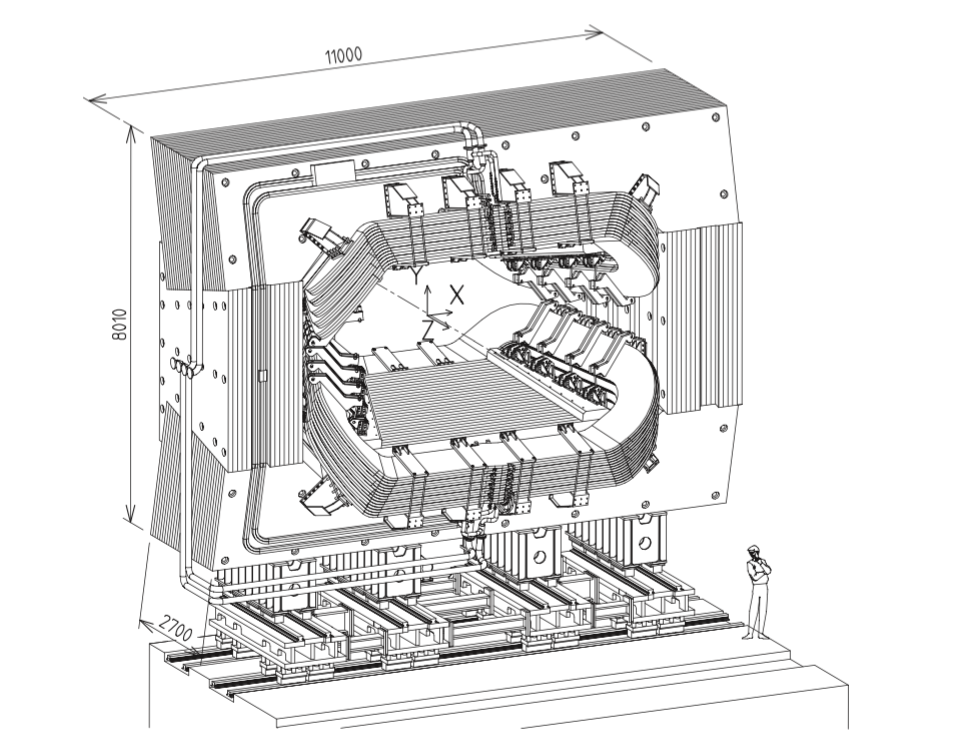
\includegraphics[ width=1.0\textwidth]{./Figs/LHC_LHCb/Magnet_picture.png}
  \caption{Magnet picture. Source: \cite{Alves:2008zz}.}
  \label{fig:types_of_tracks}
\end{figure}

\begin{figure}[tb] 
  \centering    
  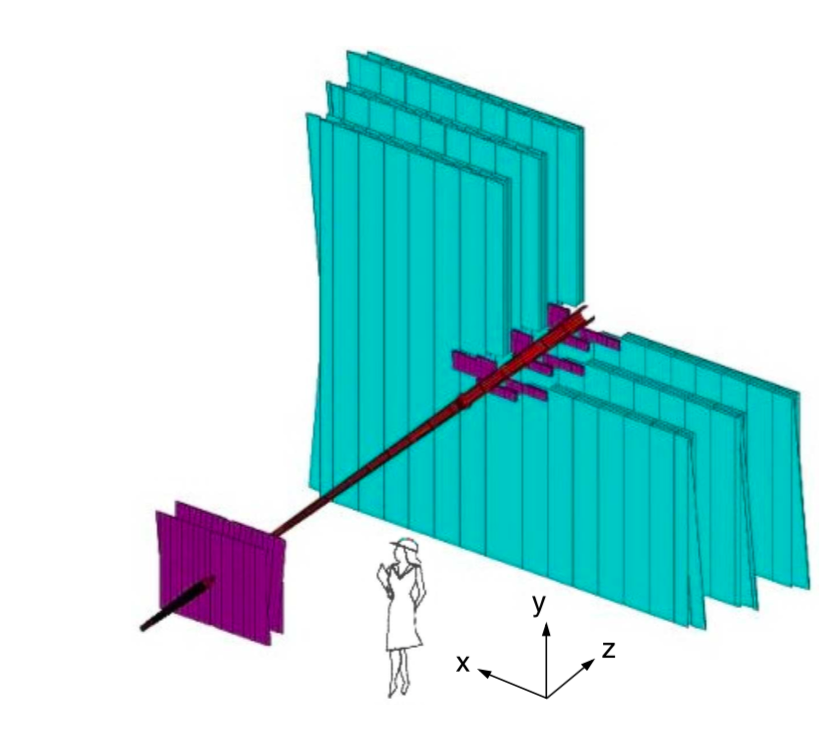
\includegraphics[ width=1.0\textwidth]{./Figs/LHC_LHCb/TT_IT_OT_comparison.png}
  \caption{TT, IT, OT comparison. Source: \cite{Alves:2008zz}.}
  \label{fig:types_of_tracks}
\end{figure}

\begin{figure}[tb] 
  \centering    
  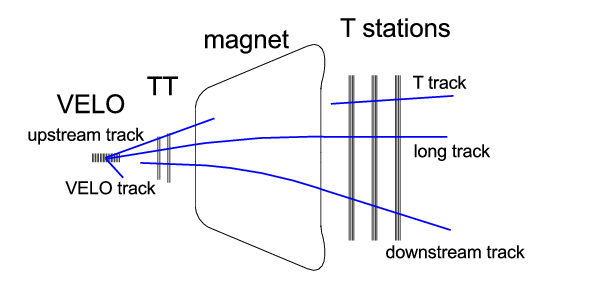
\includegraphics[ width=1.0\textwidth]{./Figs/LHC_LHCb/Types_of_tracks.png}
  \caption{Source: \cite{Aaij:2014pwa}.}
  \label{fig:types_of_tracks}
\end{figure}



\begin{figure}[tb] 
  \centering    
  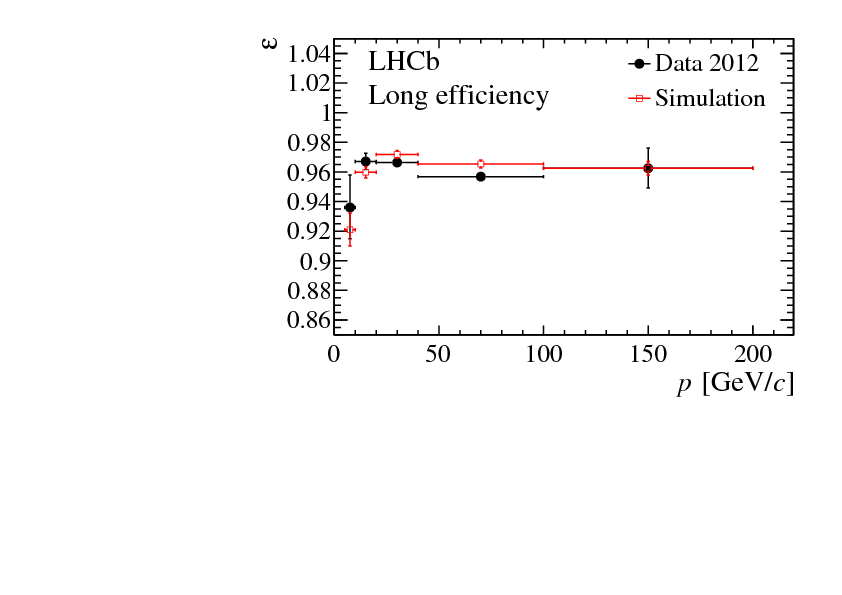
\includegraphics[ width=1.0\textwidth]{./Figs/LHC_LHCb/Long_track_efficiency_wrt_p.png}
  \caption{Source: \cite{Aaij:2014pwa}. There is also 2010 and 2011, and other variables so prehaps put no image and just says it's around 96$\%$ for Run 1.}
  \label{fig:types_of_tracks}
\end{figure}





\begin{figure}[tb] 
  \centering    
  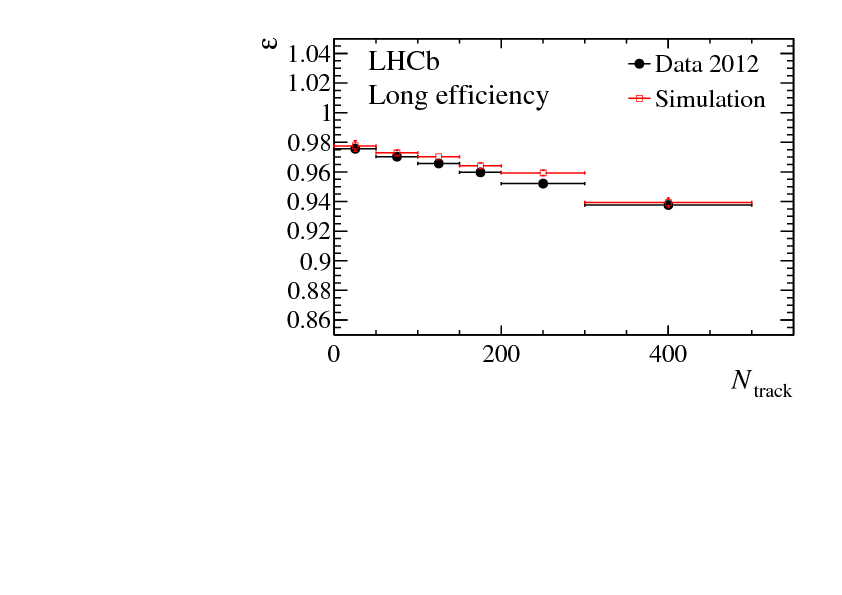
\includegraphics[ width=1.0\textwidth]{./Figs/LHC_LHCb/Long_track_efficiency_wrt_Ntracks.png}
  \caption{Source: \cite{Aaij:2014pwa}.There is also 2010 and 2011, and other variables so prehaps put no image and just says it's around 96$\%$ for Run 1.}
  \label{fig:types_of_tracks}
\end{figure}



\begin{figure}[tb] 
  \centering    
  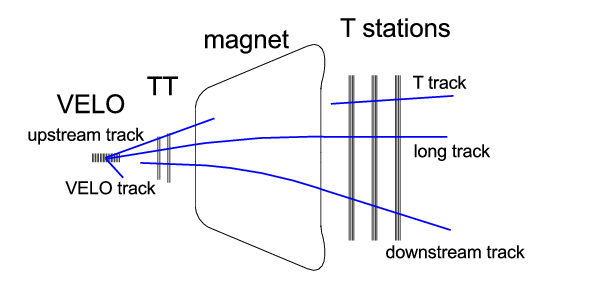
\includegraphics[ width=1.0\textwidth]{./Figs/LHC_LHCb/Types_of_tracks.png}
  \caption{Velo performance Source: \cite{}.}
  \label{fig:types_of_tracks}
\end{figure}




\subsection{Particle Identification}
\subsubsection{RICH}
\subsubsection{Calrimeters}
\subsubsection{Muon Stations}
\subsubsection{Combined PID information and performance}

\subsection{Trigger and event filtering}

\subsection{MC and Software}

\subsection{LHCb data collected so far}

\begin{figure}[tb] 
  \centering    
  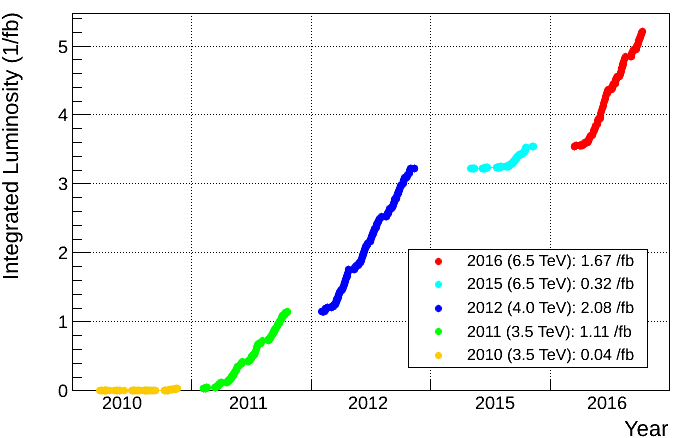
\includegraphics[ width=1.0\textwidth]{./Figs/LHC_LHCb/IntegratedLumiCumul.png}
  \caption{Source: LHCb.}
  \label{fig:cumulative_lumi}
\end{figure}

\begin{figure}[tb] 
  \centering    
  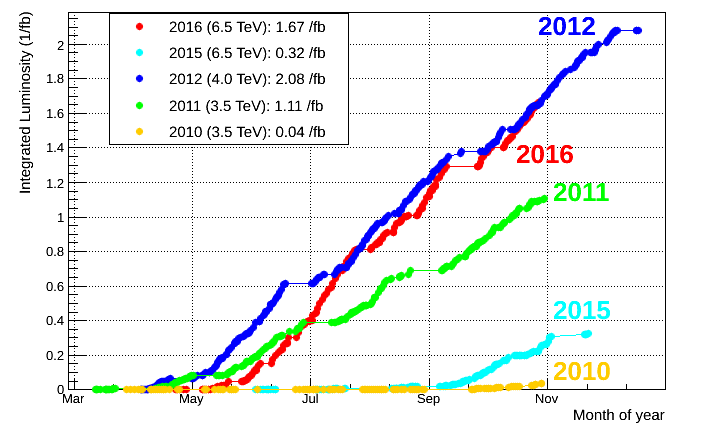
\includegraphics[ width=1.0\textwidth]{./Figs/LHC_LHCb/IntLumiRun1-2.png}
  \caption{Source: LHCb.}
  \label{fig:yearly_lumi}
\end{figure}
